\documentclass[11pt,a4paper]{article}

% Packages
\usepackage[margin=2.5cm]{geometry}
\usepackage{microtype}
\usepackage{graphicx}
\usepackage{tikz}
\usetikzlibrary{shapes,arrows.meta,positioning,calc,fit,backgrounds,shadows.blur,decorations.pathmorphing,decorations.pathreplacing}
\usepackage{colortbl}
\usepackage{enumitem}
\usepackage{booktabs}
\usepackage{longtable}
\usepackage{hyperref}
\usepackage{xcolor}
\usepackage{fancyhdr}
\usepackage{titlesec}
\usepackage[most]{tcolorbox}
\usepackage{multicol}
\usepackage{amsmath,amssymb}
\usepackage{multirow}
\usepackage{setspace}
\usepackage{fontawesome5}
\usepackage{listings}

% Spacing
\setlength{\parskip}{3pt plus 1pt minus 1pt}
\setlength{\parindent}{0pt}

% Colors
\definecolor{primary}{HTML}{0E4D64}
\definecolor{secondary}{HTML}{137177}
\definecolor{accent}{HTML}{C84B31}
\definecolor{lightbg}{HTML}{E8F6F3}
\definecolor{defbg}{HTML}{FDF2E9}
\definecolor{greenhl}{HTML}{2E8B57}
\definecolor{purplehl}{HTML}{6C5B7B}
\definecolor{codebg}{HTML}{F4F6F7}

% Hyperref
\hypersetup{colorlinks=true, linkcolor=primary, urlcolor=secondary, citecolor=primary}

% Code listings style
\lstset{
  backgroundcolor=\color{codebg},
  basicstyle=\ttfamily\small,
  keywordstyle=\color{primary}\bfseries,
  stringstyle=\color{greenhl},
  commentstyle=\color{gray},
  breaklines=true,
  frame=l,
  framerule=2pt,
  rulecolor=\color{secondary!40},
  xleftmargin=8pt,
  framexleftmargin=6pt,
  aboveskip=6pt,
  belowskip=6pt
}

% Header/Footer
\pagestyle{fancy}
\fancyhf{}
\fancyhead[L]{\small\textcolor{primary}{\textbf{Cloud Computing --- Data Science for BSIT}}}
\fancyhead[R]{\small\textcolor{primary}{Lecture Handout}}
\fancyfoot[C]{\small\thepage}
\renewcommand{\headrulewidth}{0.5pt}
\renewcommand{\footrulewidth}{0.3pt}

% Section formatting
\titleformat{\section}{\Large\bfseries\color{primary}}{\thesection}{0.6em}{}[\vspace{2pt}\titlerule]
\titleformat{\subsection}{\large\bfseries\color{secondary}}{\thesubsection}{0.5em}{}
\titleformat{\subsubsection}{\normalsize\bfseries\color{primary}}{\thesubsubsection}{0.5em}{}
\titlespacing*{\section}{0pt}{14pt}{8pt}
\titlespacing*{\subsection}{0pt}{10pt}{5pt}

% Custom boxes
\newtcolorbox{definitionbox}[1][] {
  enhanced, breakable,
  colback=defbg, colframe=orange!60!black,
  colbacktitle=orange!70!black, coltitle=white,
  title={\faIcon{book}~#1}, fonttitle=\bfseries,
  boxrule=0pt, leftrule=4pt, arc=2pt,
  shadow={1mm}{-1mm}{0mm}{black!15},
  top=4pt, bottom=4pt, left=8pt, right=8pt
}
\newtcolorbox{conceptbox}[1][] {
  enhanced, breakable,
  colback=lightbg, colframe=secondary,
  colbacktitle=secondary, coltitle=white,
  title={\faIcon{lightbulb}~#1}, fonttitle=\bfseries,
  boxrule=0pt, leftrule=4pt, arc=2pt,
  shadow={1mm}{-1mm}{0mm}{black!15},
  top=4pt, bottom=4pt, left=8pt, right=8pt
}
\newtcolorbox{alertbox}[1][] {
  enhanced, breakable,
  colback=red!4, colframe=accent,
  colbacktitle=accent, coltitle=white,
  title={\faIcon{exclamation-triangle}~#1}, fonttitle=\bfseries,
  boxrule=0pt, leftrule=4pt, arc=2pt,
  shadow={1mm}{-1mm}{0mm}{black!12},
  top=3pt, bottom=3pt, left=8pt, right=8pt
}
\newtcolorbox{examplebox}[1][] {
  enhanced, breakable,
  colback=green!4, colframe=greenhl,
  colbacktitle=greenhl, coltitle=white,
  title={\faIcon{code}~#1}, fonttitle=\bfseries,
  boxrule=0pt, leftrule=4pt, arc=2pt,
  shadow={1mm}{-1mm}{0mm}{black!12},
  top=3pt, bottom=3pt, left=8pt, right=8pt
}

\begin{document}

% Title
\begin{center}
\vspace*{0.5cm}
{\Huge\bfseries\textcolor{primary}{Cloud Computing}}\\[8pt]
{\Huge\bfseries\textcolor{primary}{Foundations for Data Science}}\\[16pt]
{\color{secondary}\rule{0.68\textwidth}{1.5pt}}\\[12pt]
{\Large\textsc{BSIT Lecture Handout}}\\[6pt]
{\large\textcolor{gray!70!black}{Course: Data Science \quad Program: BSIT}}\\[8pt]
{\normalsize\textcolor{gray!70!black}{Infrastructure \textbullet\ Data Pipelines \textbullet\ Analytics Platforms \textbullet\ Security \textbullet\ Cost}}
\vspace{0.3cm}
\end{center}

\tableofcontents
\newpage

%=============================================================
\section{Introduction to Cloud Computing}
%=============================================================

\begin{definitionbox}[Cloud Computing]
Cloud computing is the on-demand delivery of computing services such as servers, storage, databases, networking, analytics, and software over the internet. Instead of buying and maintaining all infrastructure locally, organizations rent resources when needed and pay only for what they use.
\end{definitionbox}

\begin{conceptbox}[Why It Matters in Data Science]
Modern data science depends on large datasets, collaborative tools, scalable compute, and rapid experimentation. Cloud platforms make it possible to train models, store data lakes, deploy dashboards, and serve predictions without building a large physical data center.
\end{conceptbox}

\subsection{Core Characteristics of Cloud Computing}

\begin{itemize}[leftmargin=*]
  \item \textbf{On-demand self-service:} Users provision compute, storage, and analytics resources when needed.
  \item \textbf{Broad network access:} Services are reachable through the internet from laptops, mobile devices, and APIs.
  \item \textbf{Resource pooling:} Shared infrastructure serves multiple customers efficiently through virtualization.
  \item \textbf{Rapid elasticity:} Capacity scales up or down quickly depending on workload intensity.
  \item \textbf{Measured service:} Usage is monitored for billing, governance, and performance management.
\end{itemize}

\subsection{Traditional IT vs. Cloud Model}

\begin{center}
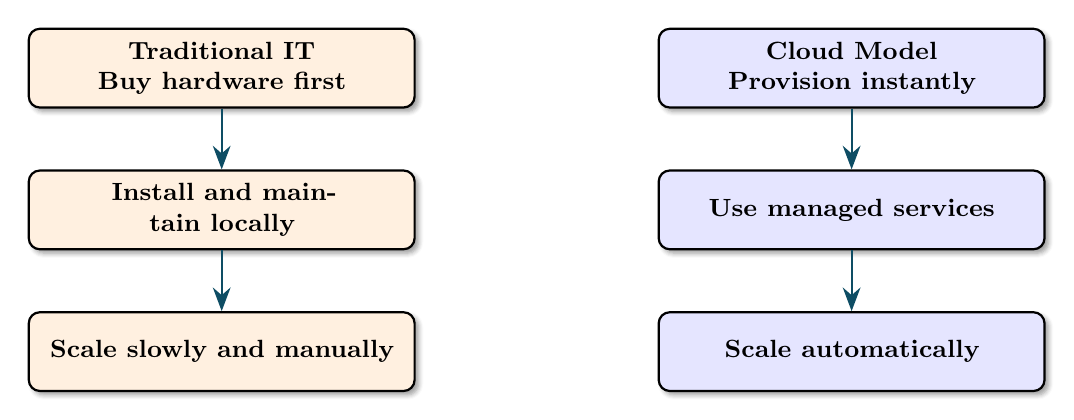
\begin{tikzpicture}[
  box/.style={rectangle, draw, thick, rounded corners=4pt, minimum width=4.9cm, minimum height=1.0cm, align=center, font=\small\bfseries,
    blur shadow={shadow blur steps=5, shadow xshift=0.5mm, shadow yshift=-0.5mm}},
  arr/.style={-{Stealth[length=3mm]}, thick, primary}
]
  \node[box, fill=orange!12, text width=4.4cm] (trad1) at (0,0) {Traditional IT\\Buy hardware first};
  \node[box, fill=orange!12, text width=4.4cm] (trad2) at (0,-1.8) {Install and maintain locally};
  \node[box, fill=orange!12, text width=4.4cm] (trad3) at (0,-3.6) {Scale slowly and manually};

  \node[box, fill=blue!10, text width=4.4cm] (cloud1) at (8,0) {Cloud Model\\Provision instantly};
  \node[box, fill=blue!10, text width=4.4cm] (cloud2) at (8,-1.8) {Use managed services};
  \node[box, fill=blue!10, text width=4.4cm] (cloud3) at (8,-3.6) {Scale automatically};

  \draw[arr] (trad1) -- (trad2);
  \draw[arr] (trad2) -- (trad3);
  \draw[arr] (cloud1) -- (cloud2);
  \draw[arr] (cloud2) -- (cloud3);
\end{tikzpicture}
\end{center}

\subsection{Why Organizations Move to the Cloud}

\begin{itemize}[leftmargin=*]
  \item Lower upfront capital expenditure.
  \item Faster deployment of software products and data platforms.
  \item Better collaboration for distributed teams.
  \item Easier disaster recovery and backup planning.
  \item Access to advanced AI, analytics, and managed database services.
\end{itemize}

%=============================================================
\section{Service Models and Deployment Models}
%=============================================================

\subsection{Cloud Service Models}

\begin{center}
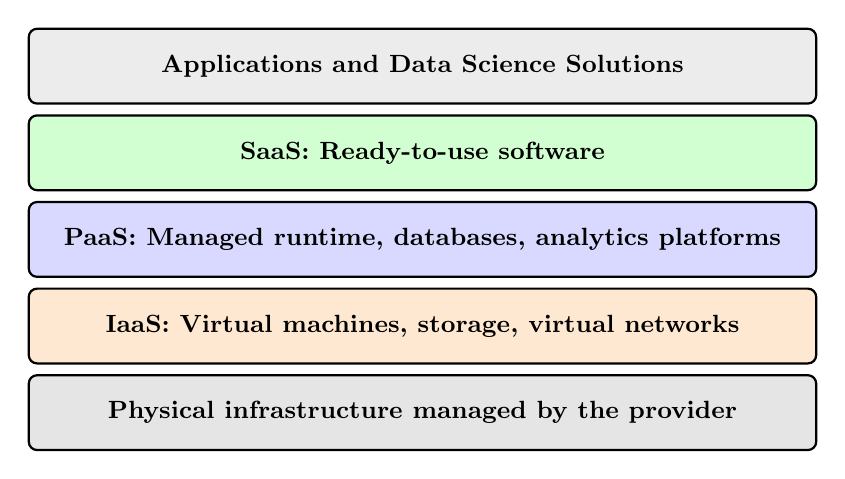
\begin{tikzpicture}[
  layer/.style={rectangle, draw, thick, minimum width=10cm, minimum height=0.95cm, align=center, font=\small\bfseries, rounded corners=3pt},
  note/.style={font=\small}
]
  \node[layer, fill=gray!15] (user) at (0,0) {Applications and Data Science Solutions};
  \node[layer, fill=green!18] (saas) at (0,-1.1) {SaaS: Ready-to-use software};
  \node[layer, fill=blue!15] (paas) at (0,-2.2) {PaaS: Managed runtime, databases, analytics platforms};
  \node[layer, fill=orange!18] (iaas) at (0,-3.3) {IaaS: Virtual machines, storage, virtual networks};
  \node[layer, fill=gray!20] (infra) at (0,-4.4) {Physical infrastructure managed by the provider};
\end{tikzpicture}
\end{center}

\begin{longtable}{p{2.7cm}p{4.2cm}p{3.6cm}p{4.0cm}}
\toprule
\textbf{Model} & \textbf{What the provider manages} & \textbf{User focus} & \textbf{Examples} \\
\midrule
IaaS & Virtual machines, networking, disks, load balancers & Operating systems, apps, data, security configuration & Azure VMs, Amazon EC2, Google Compute Engine \\
PaaS & Runtime, scaling, patching, middleware, deployment platform & Application logic, model code, data products & Azure App Service, Google App Engine, Heroku \\
SaaS & Complete application & Usage, configuration, access control, data input & Microsoft 365, Gmail, Power BI Service \\
\bottomrule
\end{longtable}

\subsection{Deployment Models}

\begin{itemize}[leftmargin=*]
  \item \textbf{Public cloud:} Resources run in infrastructure owned by a cloud provider and shared across tenants.
  \item \textbf{Private cloud:} Cloud-like environment dedicated to a single organization.
  \item \textbf{Hybrid cloud:} Combines on-premises systems with public cloud services.
  \item \textbf{Multi-cloud:} Uses services from more than one public cloud provider.
\end{itemize}

\begin{examplebox}[Choosing a Model]
A university analytics team may keep student records in a private environment for compliance, but train machine learning models in a public cloud GPU environment. This is a typical \textbf{hybrid cloud} pattern.
\end{examplebox}

%=============================================================
\section{Cloud Building Blocks for Data Science}
%=============================================================

\subsection{Essential Infrastructure Components}

\begin{multicols}{2}
\begin{itemize}[leftmargin=1.2em]
  \item \textbf{Compute:} Virtual machines, containers, serverless functions, GPU instances.
  \item \textbf{Storage:} Object storage, block storage, file shares, archives.
  \item \textbf{Databases:} Relational, NoSQL, graph, time-series, and data warehouses.
  \item \textbf{Networking:} Virtual networks, subnets, DNS, gateways, firewalls, CDNs.
  \item \textbf{Identity:} Users, service accounts, roles, policies, secrets.
  \item \textbf{Monitoring:} Logs, metrics, alerts, dashboards, tracing.
\end{itemize}
\end{multicols}

\subsection{Data Science Platform Services}

\begin{conceptbox}[Typical Cloud Services Used by Data Teams]
Data science in the cloud often combines storage for raw data, notebooks for exploration, scalable compute for training, data orchestration for pipelines, feature stores, experiment tracking, and managed endpoints for prediction serving.
\end{conceptbox}

\begin{center}
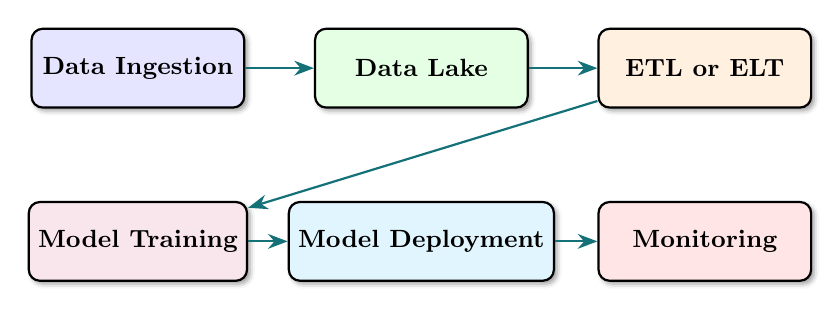
\begin{tikzpicture}[
  block/.style={rectangle, draw, thick, rounded corners=4pt, minimum width=2.7cm, minimum height=1cm, align=center, font=\small\bfseries,
    blur shadow={shadow blur steps=3, shadow xshift=0.4mm, shadow yshift=-0.4mm}},
  arr/.style={-{Stealth[length=2.5mm]}, thick, secondary}
]
  \node[block, fill=blue!10] (ingest) at (0,0) {Data Ingestion};
  \node[block, fill=green!10] (lake) at (3.6,0) {Data Lake};
  \node[block, fill=orange!12] (prep) at (7.2,0) {ETL or ELT};
  \node[block, fill=purple!10] (train) at (0,-2.2) {Model Training};
  \node[block, fill=cyan!12] (deploy) at (3.6,-2.2) {Model Deployment};
  \node[block, fill=red!10] (monitor) at (7.2,-2.2) {Monitoring};

  \draw[arr] (ingest) -- (lake);
  \draw[arr] (lake) -- (prep);
  \draw[arr] (prep) -- (train);
  \draw[arr] (train) -- (deploy);
  \draw[arr] (deploy) -- (monitor);
\end{tikzpicture}
\end{center}

\subsection{Storage Options and Use Cases}

\begin{longtable}{p{3.0cm}p{4.1cm}p{6.2cm}}
\toprule
\textbf{Storage Type} & \textbf{Purpose} & \textbf{Data Science Use Case} \\
\midrule
Object Storage & Cheap, scalable file storage & Store images, CSV files, parquet files, models, notebooks, backups \\
Block Storage & Attached disk for compute instances & High-performance training workloads on virtual machines \\
File Storage & Shared directory access & Team collaboration for scripts and intermediate outputs \\
Archive Storage & Long-term, low-cost retention & Retain old datasets or compliance backups \\
\bottomrule
\end{longtable}

%=============================================================
\section{Virtualization, Containers, and Serverless Computing}
%=============================================================

\subsection{Virtualization}

\begin{definitionbox}[Virtualization]
Virtualization is the abstraction of physical hardware into multiple virtual machines. A hypervisor allows one physical server to host many isolated computing environments.
\end{definitionbox}

\begin{itemize}[leftmargin=*]
  \item Enables efficient hardware utilization.
  \item Allows different operating systems to run on the same physical machine.
  \item Supports isolation, testing, and fast provisioning.
\end{itemize}

\subsection{Containers}

\begin{definitionbox}[Container]
A container packages application code together with its dependencies so it can run consistently across environments. Containers are lighter than virtual machines because they share the host operating system kernel.
\end{definitionbox}

\begin{itemize}[leftmargin=*]
  \item Useful for reproducible data science environments.
  \item Simplifies deployment of APIs, notebooks, and model-serving services.
  \item Common tools include Docker and Kubernetes.
\end{itemize}

\subsection{Serverless Computing}

\begin{conceptbox}[Serverless]
In serverless platforms, developers deploy functions or applications without managing servers directly. The cloud provider scales execution automatically based on demand.
\end{conceptbox}

\begin{itemize}[leftmargin=*]
  \item Best for event-driven jobs, scheduled data processing, and lightweight APIs.
  \item Pay-per-execution can reduce cost for intermittent workloads.
  \item Not ideal for long-running, memory-heavy training jobs.
\end{itemize}

\begin{examplebox}[Data Science Example]
A serverless function can automatically validate a newly uploaded CSV file, store metadata, and trigger a downstream preprocessing pipeline.
\end{examplebox}

%=============================================================
\section{Cloud Data Engineering and Analytics Workflow}
%=============================================================

\subsection{End-to-End Workflow}

\begin{center}
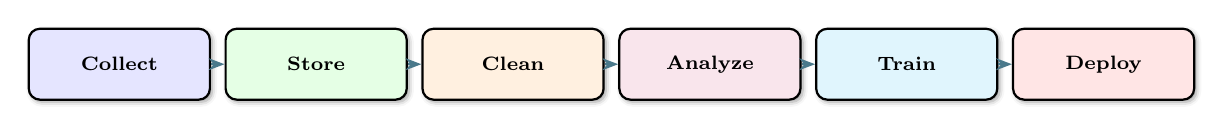
\begin{tikzpicture}[
  flowstep/.style={rectangle, draw, thick, rounded corners=4pt, minimum width=2.3cm, minimum height=0.9cm, align=center, font=\scriptsize\bfseries,
    blur shadow={shadow blur steps=3, shadow xshift=0.3mm, shadow yshift=-0.3mm}},
  arr/.style={-{Stealth[length=2mm]}, thick, primary!75}
]
  \node[flowstep, fill=blue!10] (s1) at (0,0) {Collect};
  \node[flowstep, fill=green!10] (s2) at (2.5,0) {Store};
  \node[flowstep, fill=orange!12] (s3) at (5.0,0) {Clean};
  \node[flowstep, fill=purple!10] (s4) at (7.5,0) {Analyze};
  \node[flowstep, fill=cyan!12] (s5) at (10.0,0) {Train};
  \node[flowstep, fill=red!10] (s6) at (12.5,0) {Deploy};

  \draw[arr] (s1) -- (s2);
  \draw[arr] (s2) -- (s3);
  \draw[arr] (s3) -- (s4);
  \draw[arr] (s4) -- (s5);
  \draw[arr] (s5) -- (s6);
\end{tikzpicture}
\end{center}

\subsection{Common Layers in a Cloud Data Pipeline}

\begin{itemize}[leftmargin=*]
  \item \textbf{Ingestion layer:} Collects batch or streaming data from websites, mobile apps, sensors, or business systems.
  \item \textbf{Storage layer:} Data lake or warehouse stores raw and curated data.
  \item \textbf{Processing layer:} Cleans, transforms, enriches, and aggregates data.
  \item \textbf{Analytics layer:} Supports SQL analysis, dashboards, notebooks, and reporting.
  \item \textbf{Machine learning layer:} Trains models, tracks experiments, and serves predictions.
  \item \textbf{Governance layer:} Handles identity, auditing, lineage, security, and cost tracking.
\end{itemize}

\subsection{Batch vs. Streaming Processing}

\begin{longtable}{p{3.1cm}p{5.2cm}p{5.0cm}}
\toprule
\textbf{Approach} & \textbf{Description} & \textbf{Example} \\
\midrule
Batch Processing & Data is processed at scheduled intervals & Nightly sales aggregation, weekly report generation \\
Streaming Processing & Data is processed continuously as it arrives & Fraud detection, IoT monitoring, clickstream analytics \\
\bottomrule
\end{longtable}

\begin{alertbox}[Important Design Decision]
Not every data science workload requires real-time processing. Streaming adds complexity, so teams should choose it only when low-latency insights create real business value.
\end{alertbox}

%=============================================================
\section{Security, Governance, and Reliability}
%=============================================================

\subsection{Shared Responsibility Model}

\begin{definitionbox}[Shared Responsibility]
In cloud computing, security is a shared responsibility. The provider secures the cloud infrastructure, while the customer secures identities, applications, configurations, data, and access policies.
\end{definitionbox}

\begin{itemize}[leftmargin=*]
  \item Use strong identity and access management.
  \item Encrypt data at rest and in transit.
  \item Rotate keys and secrets securely.
  \item Enable logs, alerts, and regular compliance reviews.
  \item Design backup and disaster recovery procedures.
\end{itemize}

\subsection{Security Risks in Data Science Systems}

\begin{itemize}[leftmargin=*]
  \item Misconfigured storage buckets exposing sensitive data.
  \item Weak API authentication for deployed models.
  \item Insecure notebooks containing secrets.
  \item Data poisoning or model drift in production pipelines.
  \item Over-privileged service accounts.
\end{itemize}

\subsection{Reliability Concepts}

\begin{conceptbox}[High Availability and Fault Tolerance]
Cloud systems improve reliability by replicating services across zones or regions, balancing traffic, and recovering automatically from hardware failure. For analytics systems, reliability means that pipelines, dashboards, and prediction APIs stay available even when components fail.
\end{conceptbox}

\subsection{Cost Management Principles}

\begin{itemize}[leftmargin=*]
  \item Shut down idle virtual machines and notebook sessions.
  \item Use autoscaling instead of overprovisioning.
  \item Choose storage tiers based on access frequency.
  \item Monitor data egress and inter-region transfer costs.
  \item Track experiments to avoid wasteful repeated training runs.
\end{itemize}

%=============================================================
\section{Cloud Computing Use Cases in Data Science}
%=============================================================

\subsection{Representative Applications}

\begin{itemize}[leftmargin=*]
  \item \textbf{Business intelligence:} Dashboards, KPI reporting, and descriptive analytics.
  \item \textbf{Predictive analytics:} Demand forecasting, churn prediction, and risk scoring.
  \item \textbf{Computer vision:} Image classification, object detection, quality inspection.
  \item \textbf{Natural language processing:} Sentiment analysis, chatbots, document tagging.
  \item \textbf{Recommendation systems:} Product suggestions and personalized content.
  \item \textbf{IoT analytics:} Sensor processing, anomaly detection, and predictive maintenance.
\end{itemize}

\subsection{Mini Case Study: Student Performance Analytics}

\begin{examplebox}[Scenario]
A BSIT department wants to predict which students may need academic intervention. Data from enrollment systems, attendance logs, and learning platforms is collected into a cloud data lake. A processing pipeline cleans and joins records, a machine learning model predicts risk scores, and a dashboard shows advisers the students who need support.
\end{examplebox}

\textbf{Why cloud helps:}
\begin{itemize}[leftmargin=*]
  \item Centralizes data from multiple systems.
  \item Supports collaborative notebooks for analysis.
  \item Scales model training during peak academic periods.
  \item Enables secure dashboards for administrators and advisers.
\end{itemize}

\subsection{Benefits and Challenges}

\begin{longtable}{p{5.9cm}p{5.9cm}}
\toprule
\textbf{Benefits} & \textbf{Challenges} \\
\midrule
Elastic scaling for experiments & Cost overruns from poor governance \\
Fast access to managed services & Misconfiguration and security mistakes \\
Collaboration across teams and campuses & Vendor lock-in concerns \\
Disaster recovery and backup options & Need for cloud skills and architectural discipline \\
Access to GPUs and AI services & Data privacy and regulatory requirements \\
\bottomrule
\end{longtable}

%=============================================================
\section{Cloud Skills for BSIT Data Science Students}
%=============================================================

\subsection{Technical Skills to Build}

\begin{multicols}{2}
\begin{itemize}[leftmargin=1.2em]
  \item Linux and command line basics
  \item SQL and cloud data warehouses
  \item Python for data pipelines and automation
  \item APIs and web services
  \item Containerization with Docker
  \item CI or CD basics for deployment
  \item IAM and security fundamentals
  \item Monitoring and logging concepts
\end{itemize}
\end{multicols}

\subsection{Professional Mindset}

\begin{conceptbox}[Thinking Beyond Coding]
Cloud computing in data science is not only about writing code. It also requires reasoning about scalability, security, maintainability, observability, privacy, and cost. Strong practitioners design systems that are useful, safe, and sustainable.
\end{conceptbox}

\subsection{Sample Study Roadmap}

\begin{enumerate}[leftmargin=*]
  \item Learn core networking, operating systems, and databases.
  \item Practice storing and querying data in a cloud platform.
  \item Build a simple ETL pipeline and dashboard.
  \item Containerize a machine learning API.
  \item Deploy a small end-to-end analytics project with monitoring.
\end{enumerate}

%=============================================================
\section{Key Takeaways and Review Questions}
%=============================================================

\subsection{Key Takeaways}

\begin{itemize}[leftmargin=*]
  \item Cloud computing provides scalable, on-demand infrastructure and managed services.
  \item Data science teams rely on cloud platforms for storage, processing, experimentation, and deployment.
  \item IaaS, PaaS, and SaaS represent different levels of abstraction and management responsibility.
  \item Security, governance, and cost optimization are part of every cloud architecture decision.
  \item BSIT students should connect cloud knowledge with data engineering, analytics, and machine learning practice.
\end{itemize}

\subsection{Review Questions}

\begin{enumerate}[leftmargin=*]
  \item What are the five essential characteristics of cloud computing?
  \item How do IaaS, PaaS, and SaaS differ from one another?
  \item Why is cloud computing useful for data science workflows?
  \item When would you choose batch processing over streaming processing?
  \item What does the shared responsibility model mean in cloud security?
  \item How can poor cloud governance affect the cost of a project?
\end{enumerate}

\begin{examplebox}[Short Reflection Task]
Design a simple cloud-based data science solution for one problem in your school or local community. Identify the data source, storage layer, analysis tool, model or dashboard output, and one security control you would apply.
\end{examplebox}

\vfill
\begin{center}
{\large\textcolor{primary}{\textbf{End of Handout}}}\\[4pt]
{\small\textcolor{gray!70!black}{Cloud Computing for Data Science --- BSIT Program}}
\end{center}

\end{document}